Cette exercice est un questionnaire à choix multiples. Pour chacune des six questions suivantes, une seule des quatre réponses proposées est exacte.

Une réponse fausse, une réponse multiple ou l'absence de réponse à une question ne rapporte ni n'enlève de point.

Pour répondre, indiquer sur la copie le numéro de la question et la lettre de la réponse choisie. Aucune justification n'est demandée.

\begin{enumerate}
	\item On considère  la fonction $g$ définie est dérivable sur $\intervOO{0}{+\infty}$ par $g(x) = \ln \left(x^2 + x + 1\right)$.
	
	Pour tout nombre réel $x$ strictement positif :
	
	\begin{tblr}{width=\linewidth,colspec={X[l]X[l]}}
		(a)~~$g'(x) = \dfrac{1}{2x + 1}$&(b)~~$g'(x) = \dfrac{1}{x^2 + x + 1}$\\
		(c)~~$g'(x) = \ln (2x + 1)$&(d)~~$g'(x) = \dfrac{2x + 1}{x^2 + x + 1}$
	\end{tblr}
	\item La fonction $x \mapsto \ln (x)$ admet pour primitive sur $\intervOO{0}{+\infty}$ la fonction :
	
	\begin{tblr}{width=\linewidth,colspec={X[l]X[l]X[l]X[l]}}
		(a)~~$x \mapsto \ln (x)$&(b)~~$x \mapsto \dfrac{1}{x}$&(c)~~$x \mapsto x \ln (x) - x$&(d)~~$x \mapsto \dfrac{\ln (x)}{x}$
	\end{tblr}
	\item On considère la suite $\left(a_n\right)$ définie  pour tout $n$ dans $\N$ par $a_n = \dfrac{1 - 3^n}{1 + 2^n}$.
	
	La limite de la suite $\left(a_n\right)$ est égale à :
	
	\begin{tblr}{width=\linewidth,colspec={X[l]X[l]X[l]X[l]}}
		(a)~~$- \infty$&(b)~~$-1$&(c)~~$1$&(d)~~$+\infty$
	\end{tblr}
	\item On considère une fonction $f$ définie est dérivable sur $\intervFF{-2}{2}$. Le tableau de variations de la fonction $f'$ dérivée de la fonction $f$ sur l'intervalle $[2~;~2]$ est donné par :
	%
	\begin{center}
		\begin{tikzpicture}
			\tkzTabInit{$x$/1,$f$/2}{$-2$,$-1$,$0$,$2$}
			\tkzTabVar{+/$1$,R/,-/$-2$,+/$-1$}
			\tkzTabIma{1}{3}{2}{$0$}
		\end{tikzpicture}
	\end{center}
	%
	La fonction $f$ est :
	
	\begin{tblr}{width=\linewidth,colspec={X[l]X[l]}}
		(a)~~ convexe sur $\intervFF{-2}{-1}$ &(b)~~ concave sur $\intervFF{0}{1}$\\
		(c)~~ convexe sur$\intervFF{-1}{2}$&(d)~~concave sur $\intervFF{-2}{0}$
	\end{tblr}
	
	\pagebreak
	\item On donne ci-dessus la courbe représentative de la dérivée $f'$ d'une fonction $f$ définie sur l'intervalle $\intervFF{-2}{4}$.
	%
	\begin{center}
		\begin{tikzpicture}[x=1cm,y=1cm,xmin=-2,xmax=4,xgrille=1,xgrilles=0.5,ymin=-3,ymax=3,ygrille=1,ygrilles=0.5]
			\GrilleTikz \AxesTikz[ElargirOx=0/0,ElargirOy=0/0]
			\AxexTikz[Police=\small]{-2,-1,...,3} \AxeyTikz[Police=\small]{-3,-2,...,2}
			\clip (\xmin,\ymin) rectangle (\xmax,\ymax) ;
			\draw[samples=250,domain=\xmin:\xmax,very thick,blue] plot (\x,{0.5*\x*\x*\x - 1.5*\x*\x + 1}) ;
		\end{tikzpicture}
	\end{center}
	%
	Par lecture graphique de la courbe de $f'$, déterminer l'affirmation correcte pour $f$ :
	
	\begin{tblr}{width=\linewidth,colspec={X[l]X[l]}}
		(a)~~$f$ est décroissante sur $\intervFF{0}{2}$&(b)~~$f$ est décroissante sur $\intervFF{-1}{0}$\\
		(c)~~$f$ admet un maximum en 1 sur $\intervFF{0}{2}$&(d)~~$f$ admet un maximum en 3 sur $\intervFF{2}{4}$
	\end{tblr}
	\item Une action est cotée à 57\,€. Sa valeur augmente de 3\,\% tous les mois.
	
	La fonction \textsf{Python} \texttt{seuil()} qui renvoie le nombre de mois à attendre pour que sa valeur dépasse 200\,€ est :
	
	\begin{tblr}{width=\linewidth,colspec={X[l]X[l]}}
		(a)~~&(b)~~
	\end{tblr}
	
	\begin{minipage}{0.49\linewidth}
\begin{CodePythonLstAlt}*[Largeur=0.95\linewidth]{}
def seuil() :
	m = 0
	v = 57
	while v < 200 :
		m = m+1
		v = v*1.03
	return m
\end{CodePythonLstAlt}
	\end{minipage}\hfill~
	\begin{minipage}{0.49\linewidth}
\begin{CodePythonLstAlt}*[Largeur=0.95\linewidth]{}
def seuil() :
	m = 0
	v = 57
	while v > 200 :
		m = m+1
		v = v*1.03
	return m
\end{CodePythonLstAlt}
	\end{minipage}
	
	\begin{tblr}{width=\linewidth,colspec={X[l]X[l]}}
		(c)~~&(d)~~
	\end{tblr}
	
	\begin{minipage}{0.49\linewidth}
\begin{CodePythonLstAlt}*[Largeur=0.95\linewidth]{}
def seuil() :
	v = 57
	for i in range(200):
		v = v*1.03
	return v
\end{CodePythonLstAlt}
	\end{minipage}\hfill~
	\begin{minipage}{0.49\linewidth}
\begin{CodePythonLstAlt}*[Largeur=0.95\linewidth]{}
def seuil() :
	m = 0
	v = 57
	if v < 200 :
		m = m+1
	else :
		v = v*1.03
	return m
\end{CodePythonLstAlt}
	\end{minipage}
\end{enumerate}

